\problemname{Snóker}
\illustration{0.3}{framestart}{Photo from \href{https://www.flickr.com/photos/192927703@N08/51223529455}{flickr.com}}

Arnar has been watching snooker recently.
Snooker is played on a large rectangular table and the players use a cue, which is just a custom made stick.
The play area on the table is $140.5$ inches long and $70$ inches wide.
There are six pockets on the table, one in each corner and then two others, located on the center of each of the longer sides.

There are also balls on the table in multiple colours and each colour has purpose.
The radius of each ball is $1$ inch.
The colours are red, yellow, green, brown, blue, pink and black.
Additionally, there is a white ball on the table which is the only ball players can hit with their cue.
Players then poke one end of the cue into the white ball so that it rolls on the table.
It can hit the sides of the table and bounce off of them as well as collide with the other balls.
The goal of the game is to hit the white ball into the coloured balls so that they roll into the pockets on the table, known as pocketing balls.
Hitting a ball into a pocket grants points, based on the colour, as can be seen in the following table.

\begin{center}
\begin{tabular}{|l|l|}
\hline
    Colour   & Points \\ \hline
    Red      & $1$  \\ \hline
    Yellow   & $2$  \\ \hline
    Green    & $3$  \\ \hline
    Brown    & $4$  \\ \hline
    Blue     & $5$  \\ \hline
    Pink     & $6$  \\ \hline
    Black    & $7$  \\ \hline
\end{tabular}
\end{center}

Each time the white ball is hit, a certain colour is designated as the first colour to hit with the white ball, known as the on colour.
Each time the correct colour is pocketed by a player, the player gets to hit the white ball again.
If there is a red ball on the table when a player starts their turn, then red is the on colour.
If the player pockets a red, then they can choose the on colour, except for red, for their next shot.
If the player pockets a coloured ball on that shot, then the coloured ball is placed on the table again after points have been awarded.
After that shot, the on colour is set to red again.

If the white ball hits the right colour first, then the shot is a \texttt{HIT}.
If the white ball hits the wrong colour first, then the shot is a \texttt{FOUL}.
If the white ball does not hit any ball, then the shot is a \texttt{MISS}.
Note that the white ball can hit the sides of the table as many times as possible, both before hitting a ball, and after.

One of the goals of the game is to \emph{snooker} the opponent, by hitting the white ball so it is poorly placed for the opponent.
At that point it can prove difficult to hit a correct ball, and a direct shot may not be possible.
The white ball is then usually shot so that it bounces off the sides of the table before hitting a ball.
Since it can be difficult to visualize the bounces, Arnar wants you to tell him whether the white ball hits a correct ball.

You are given the current state of the table, the on colour and a description of how the white ball will travel after being hit with the cue.
Determine whether the shot is a \texttt{HIT}, a \texttt{FOUL}, or a \texttt{MISS}.
To simplify the task, you may assume there are no pockets on the table, so the white ball cannot be pocketed, but rather always bounces off the sides upon hitting them.

\section*{Input}
The first line of input contains a single integer $n$, where $2 \leq n \leq 22$, representing the number of balls on the table.
Then $n$ lines follow.
Each line consists of the colour of the ball and two real numbers $x_i$, where $1 \leq x_i \leq 69$, and $y_i$, where $1 \leq y_i \leq 139.5$,
which represent the position of $i$-th ball.
Then a line with the on colour follows.
Finally, the input ends with a line consisting of two space separated real numbers $v_x$ and $v_y$, where $-1\,000 \leq v_x, v_y \leq 1\,000$, which represent the distance the white ball will travel on each axis.

The colours of the balls are described by the strings \texttt{white}, \texttt{red}, \texttt{yellow}, \texttt{green}, \texttt{brown}, \texttt{blue}, \texttt{pink} and \texttt{black}.
There can be up to $15$ red balls on the table, but at most $1$ of each of the other colours.
The white ball will always be on the table, as well as at least one ball with the same colour as the on colour.
The position of each ball is given as the distance from the top left corner of the table and the center of the ball, in inches.
The top left corner is therefore at the position $(0, 0)$ and the bottom right is at $(70, 140.5)$.
You may assume the balls do not intersect, but they may touch.
The white ball however will not touch any ball initially.
All real numbers are given with exactly three digits after the decimal point.

\section*{Output}
Output \texttt{HIT} if the white ball hits the correct colour first,
\texttt{FOUL} if the white ball hits the wrong colour first, or
\texttt{MISS} if the white ball does not hit any ball.
You may assume the answer will not change if the positions of the balls change by less than $10^{-3}$ inches and therefore the answer is never ambiguous.

\section*{Scoring}
\begin{tabular}{|l|l|l|}
\hline
Group & Points & Constraints \\ \hline
1     & 30     & The white ball does not travel far enough to reach a side of the table. Either $v_x = 0$ or $v_y = 0$. \\ \hline
2     & 20     & Either $v_x = 0$ or $v_y = 0$. \\ \hline
3     & 25     & The white ball does not travel far enough to reach a side of the table. \\ \hline
4     & 25     & No further constraints. \\ \hline
\end{tabular}

\section*{Explanation of samples}
The first sample belongs to group $1$. The answer is \texttt{HIT} because the white ball hits the black ball first.
\begin{figure}[ht!]
  \centering
    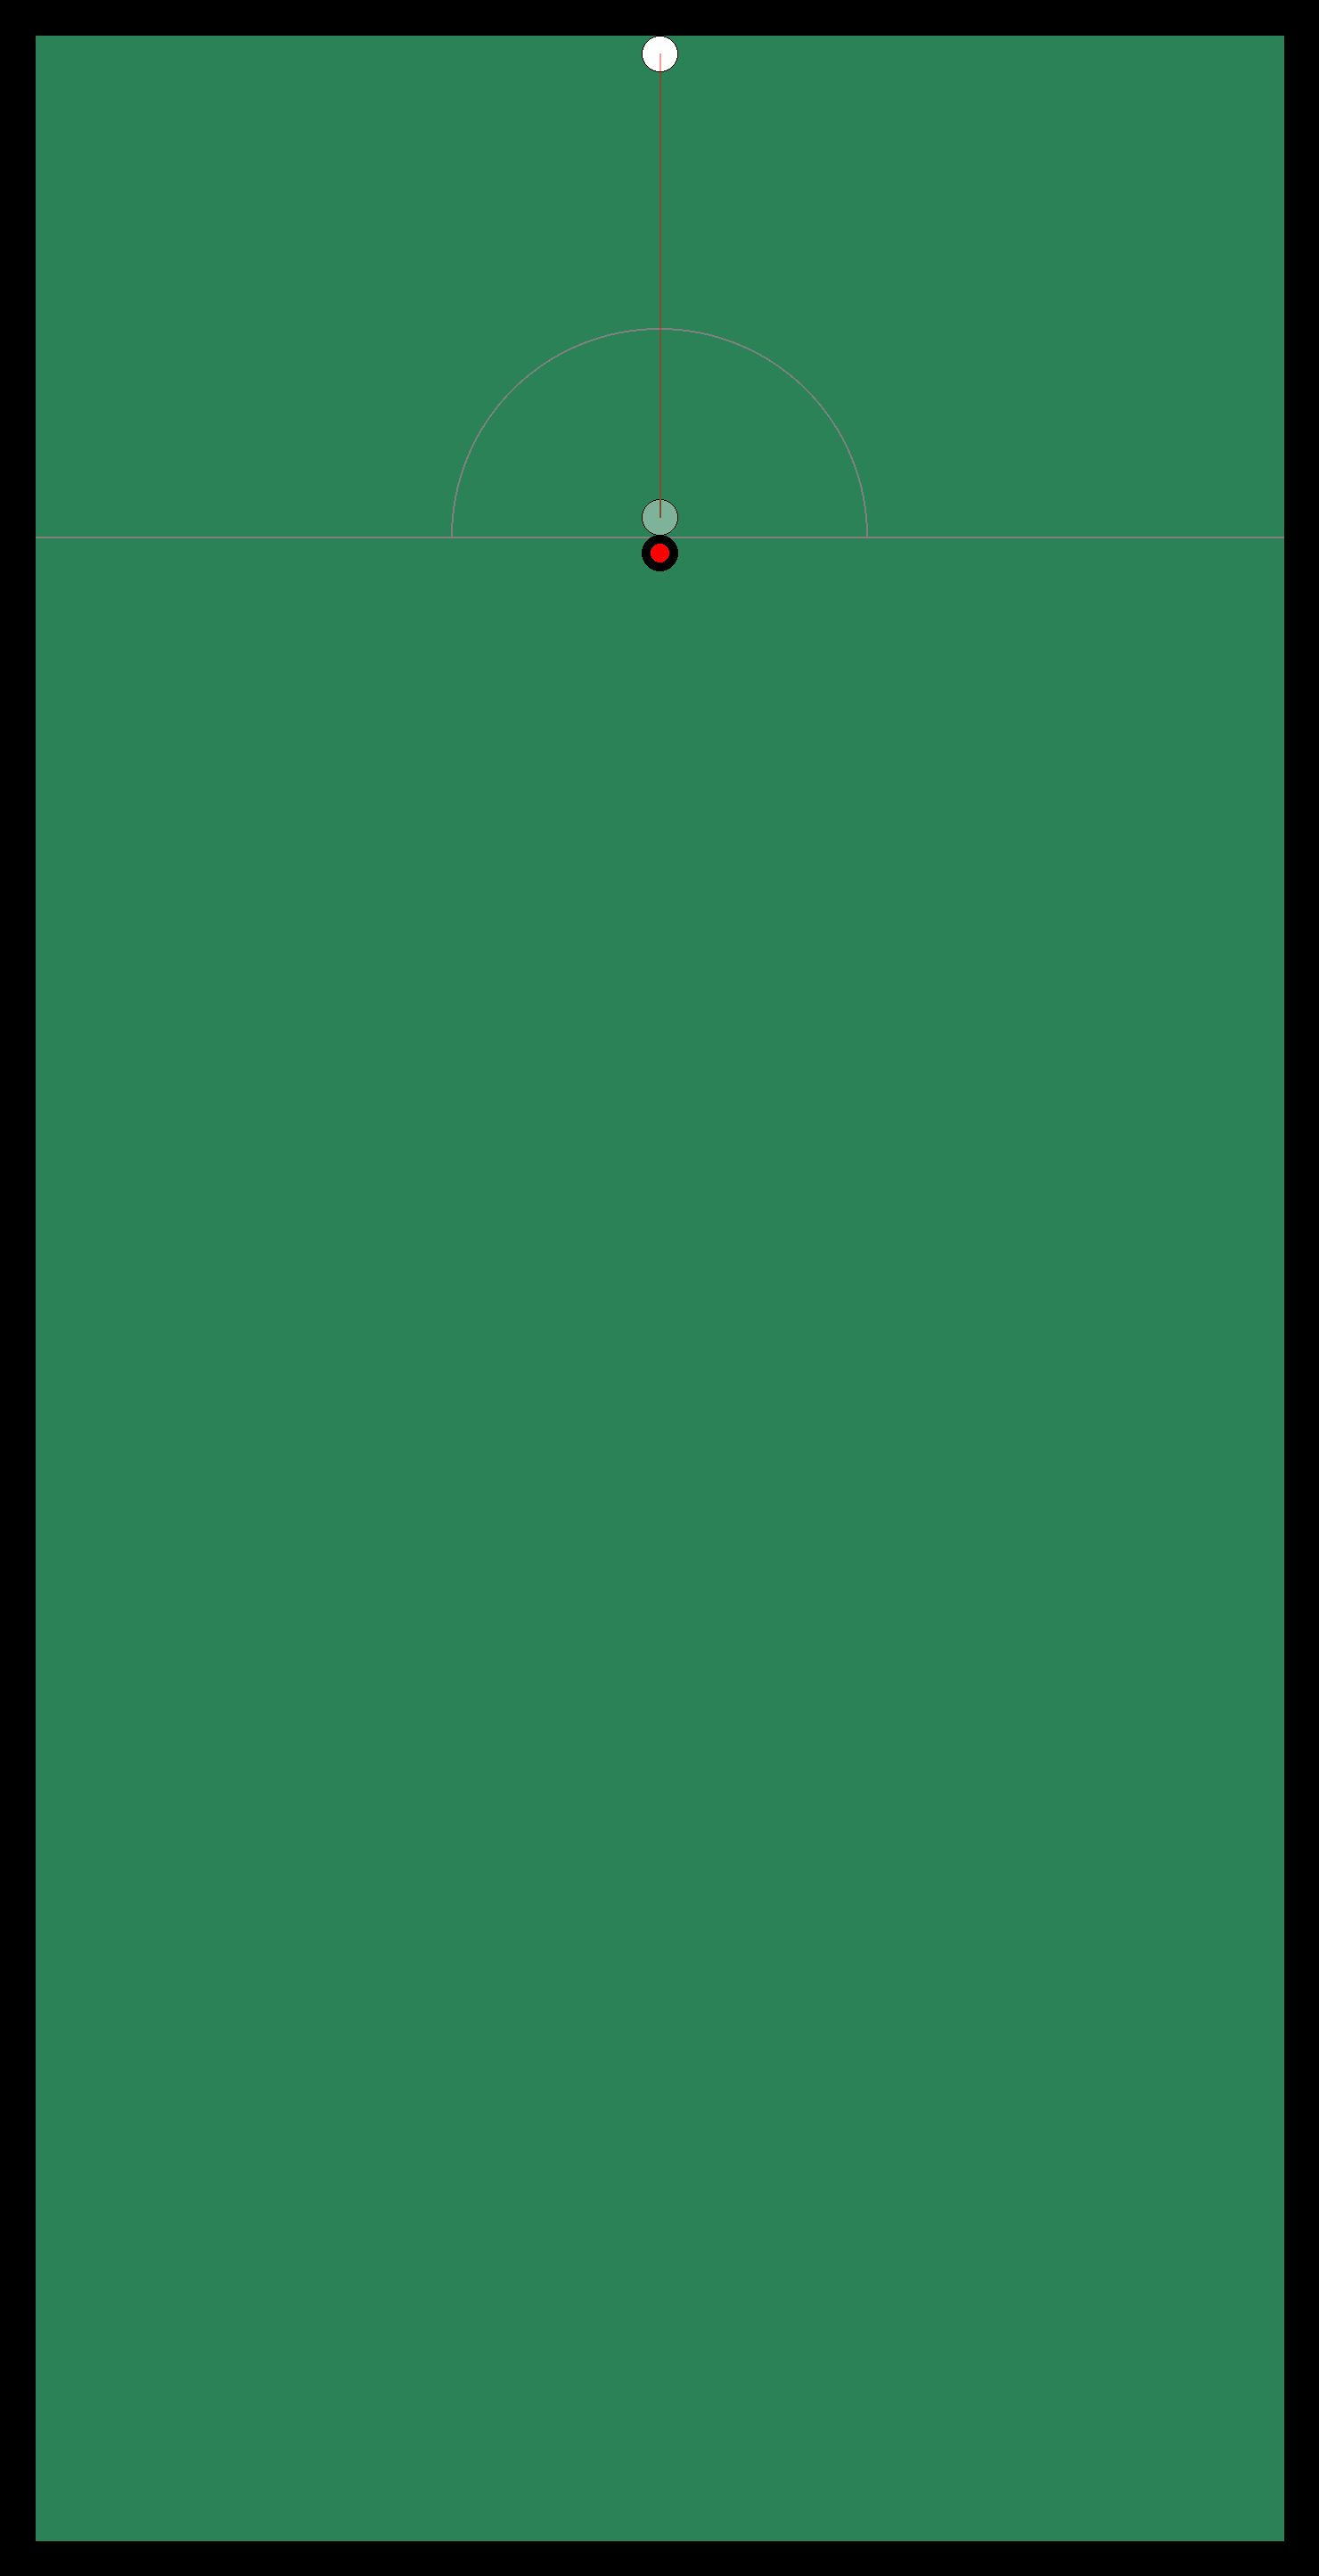
\includegraphics[width=0.7\textwidth]{sample1}
  \caption{Sample 1}
\end{figure}

The second sample belongs to group $2$. The white ball bounces of the bottom side and then travels up the table. The answer is \texttt{FOUL} because the white ball hits the pink ball first. 
\begin{figure}[ht!]
  \centering
    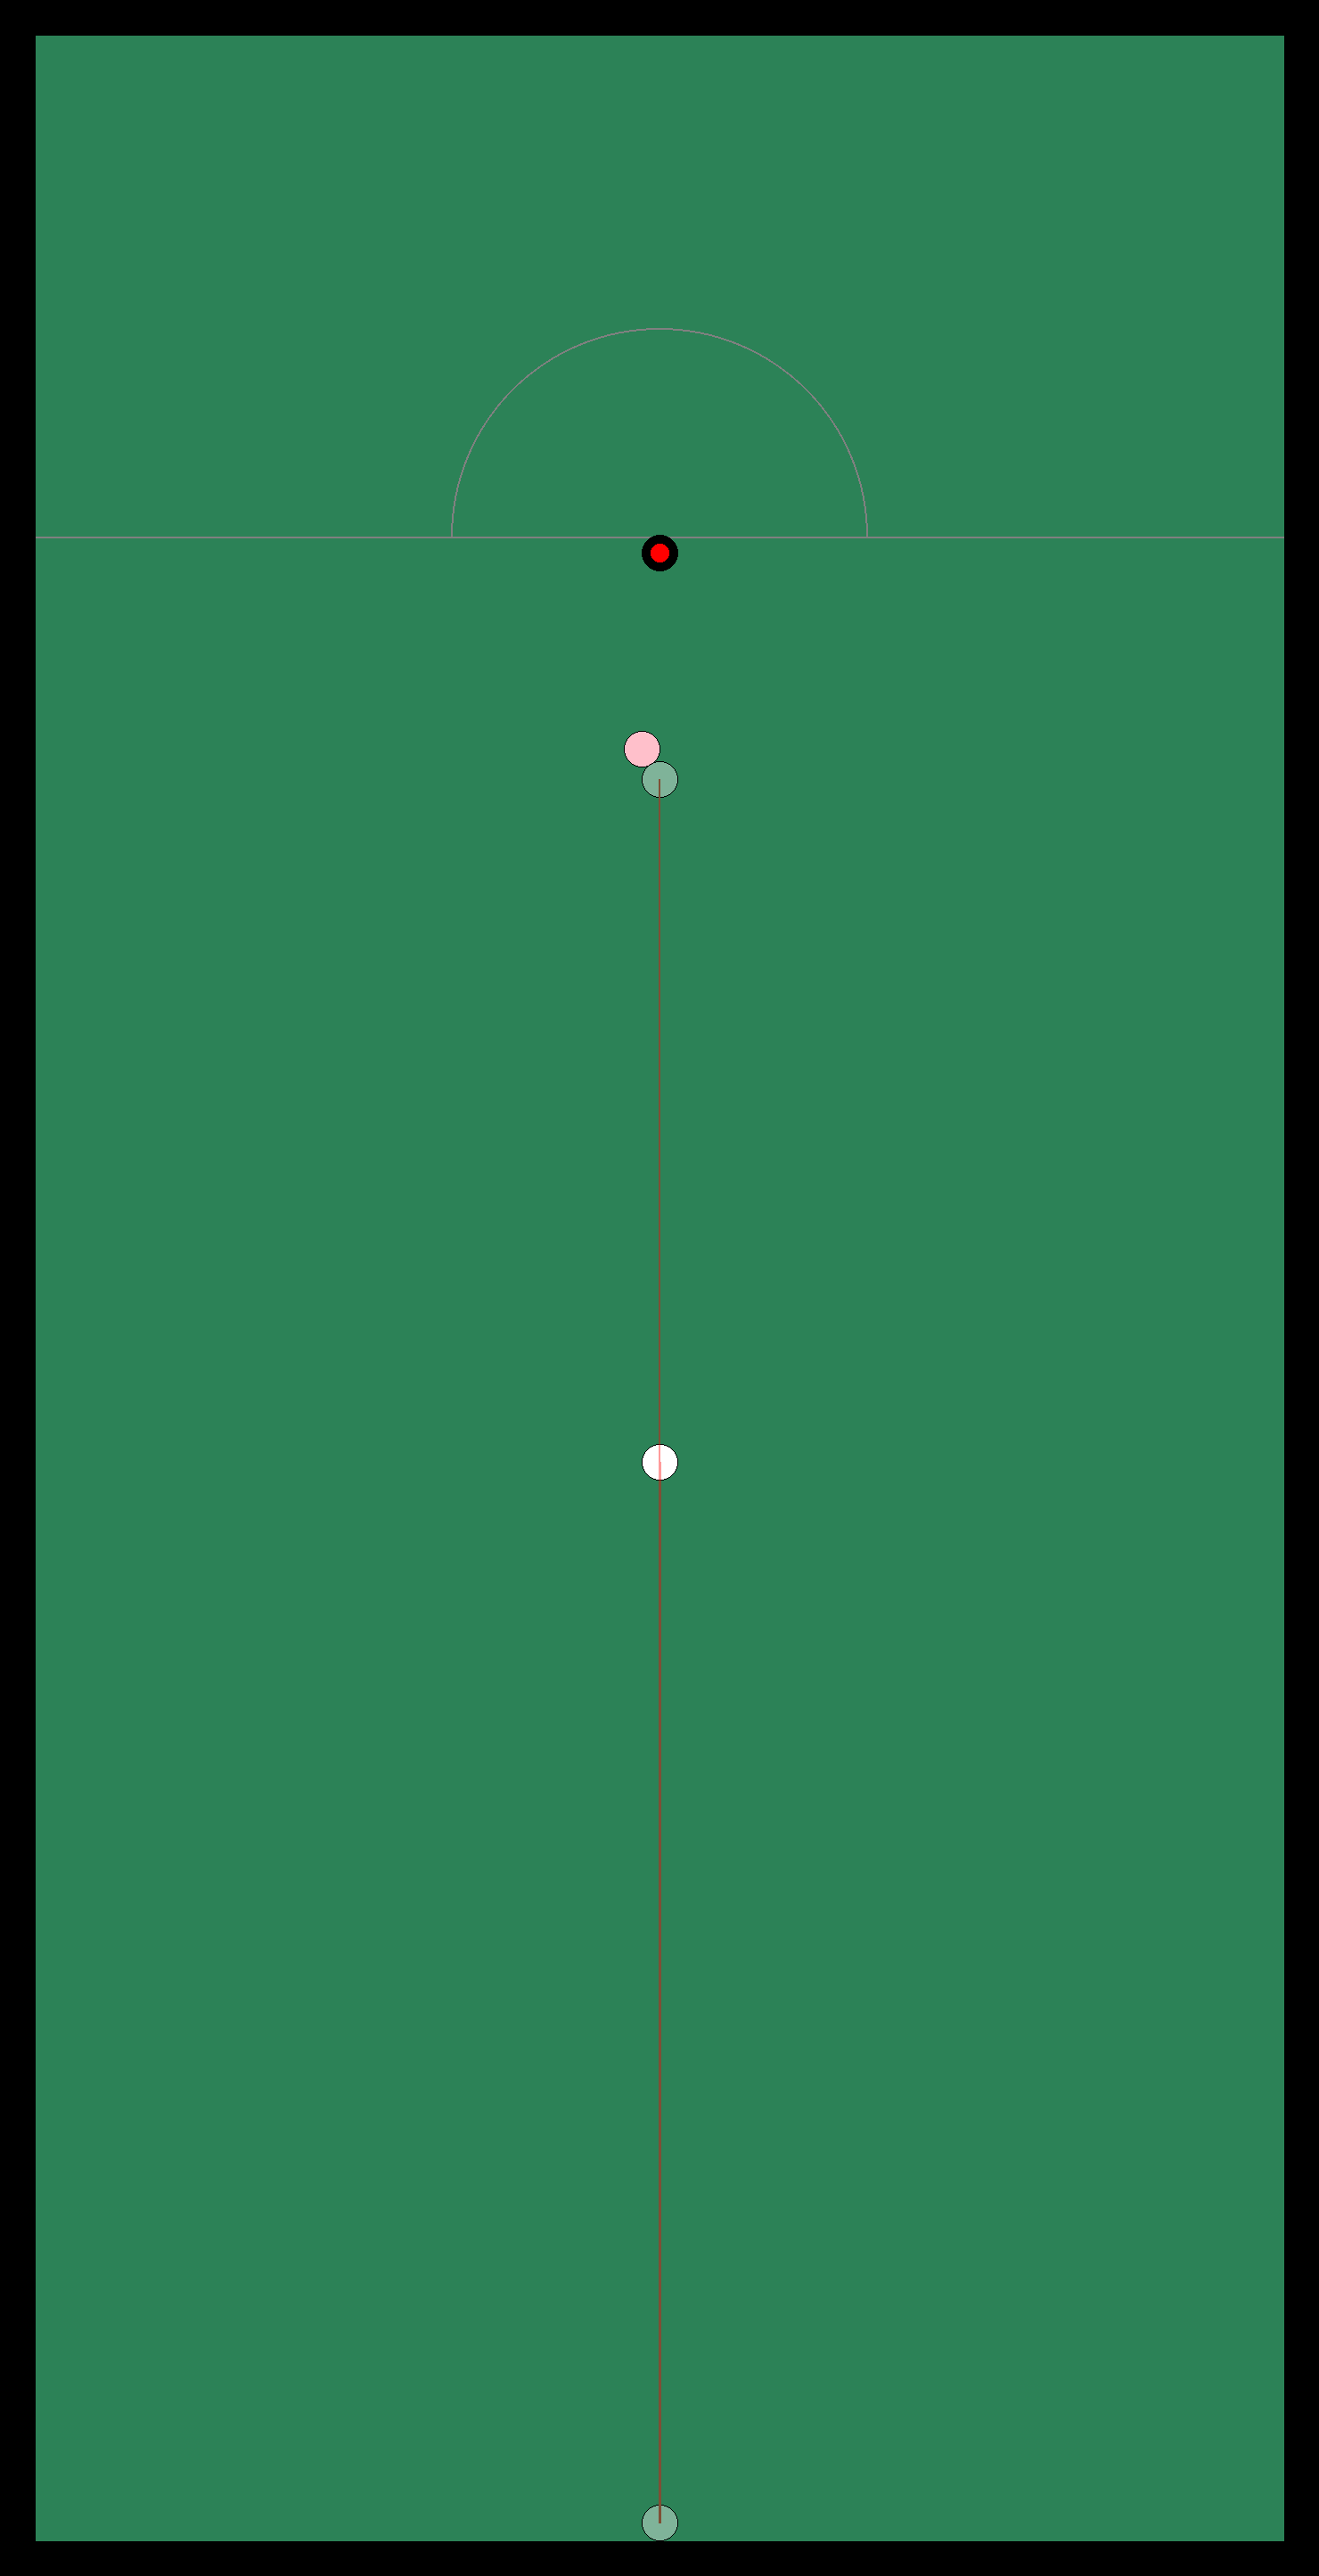
\includegraphics[width=0.7\textwidth]{sample2}
  \caption{Sample 2}
\end{figure}

The third sample belongs to group $3$. The white ball goes between the green ball and the brown ball. The answer is \texttt{FOUL} because the white ball hits the blue ball first.
\begin{figure}[ht!]
  \centering
    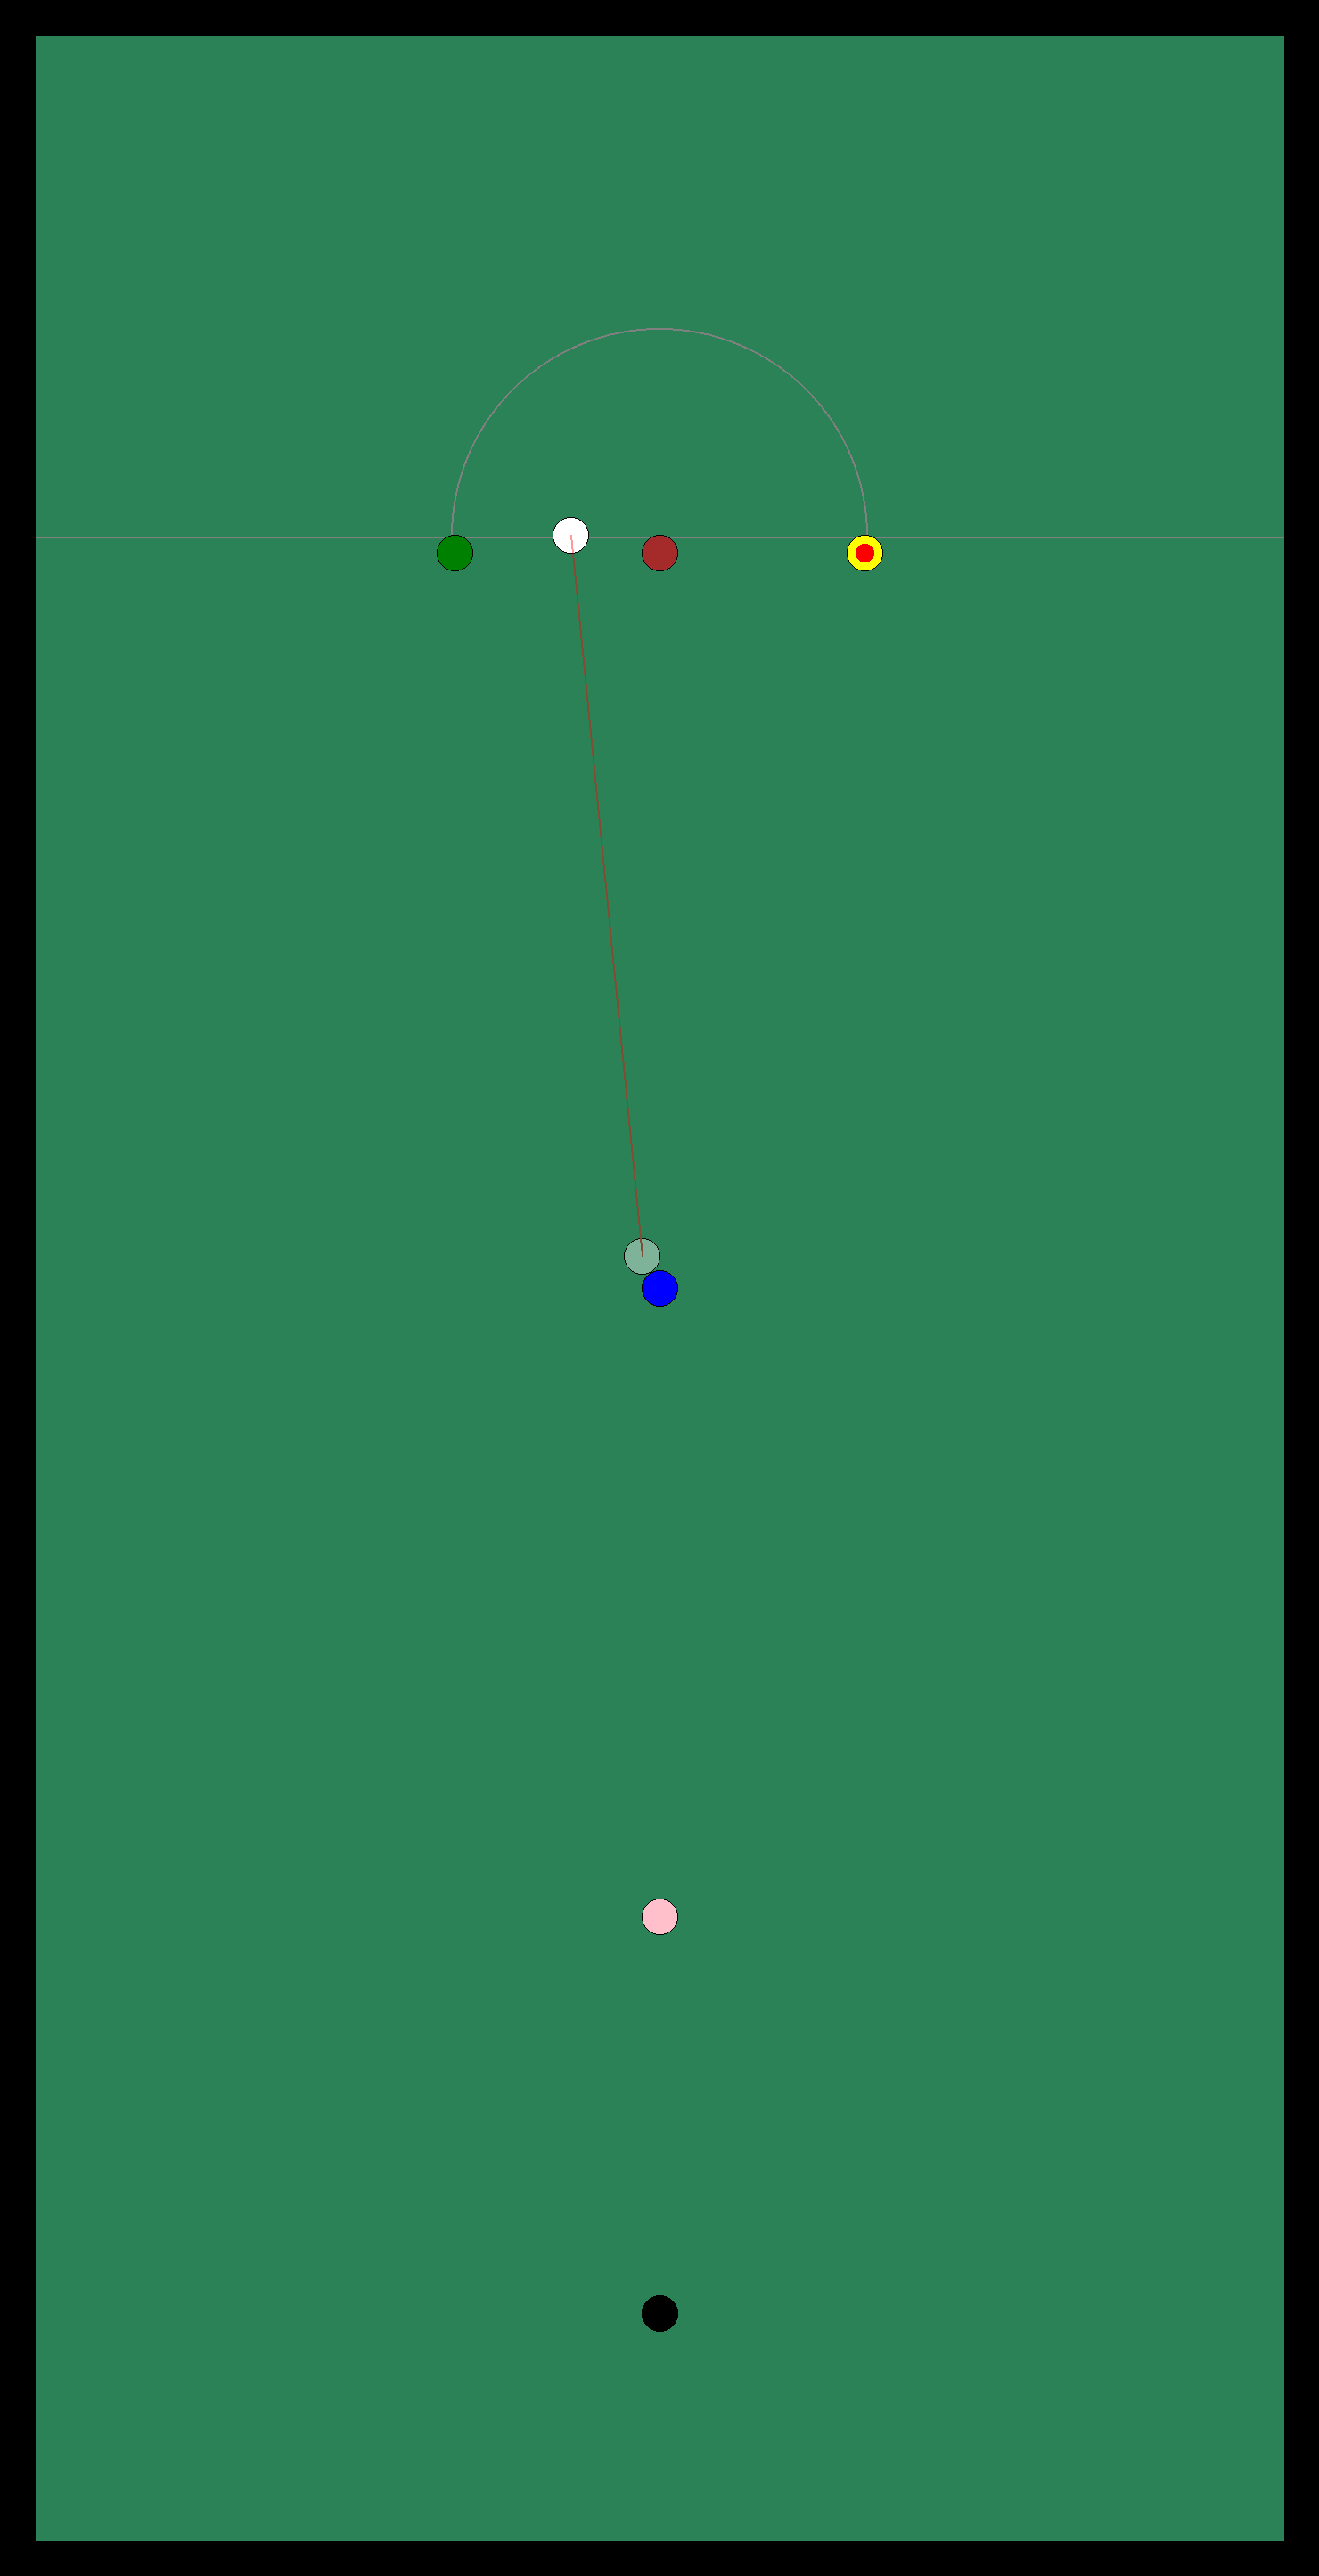
\includegraphics[width=0.7\textwidth]{sample3}
  \caption{Sample 3}
\end{figure}

The fourth sample belongs to group $4$. The white ball first travels between the brown ball and the yellow ball, bounces off the bottom side and then the left side.
Then the white ball travels past the green ball, bounces off the top side and then travels between the green ball and the brown ball.
Finally the white ball bounces off the bottom side and then comes to a stop near the right side.
The answer is \texttt{MISS} because the white ball did not hit any ball before coming to a stop.
\begin{figure}[ht!]
  \centering
    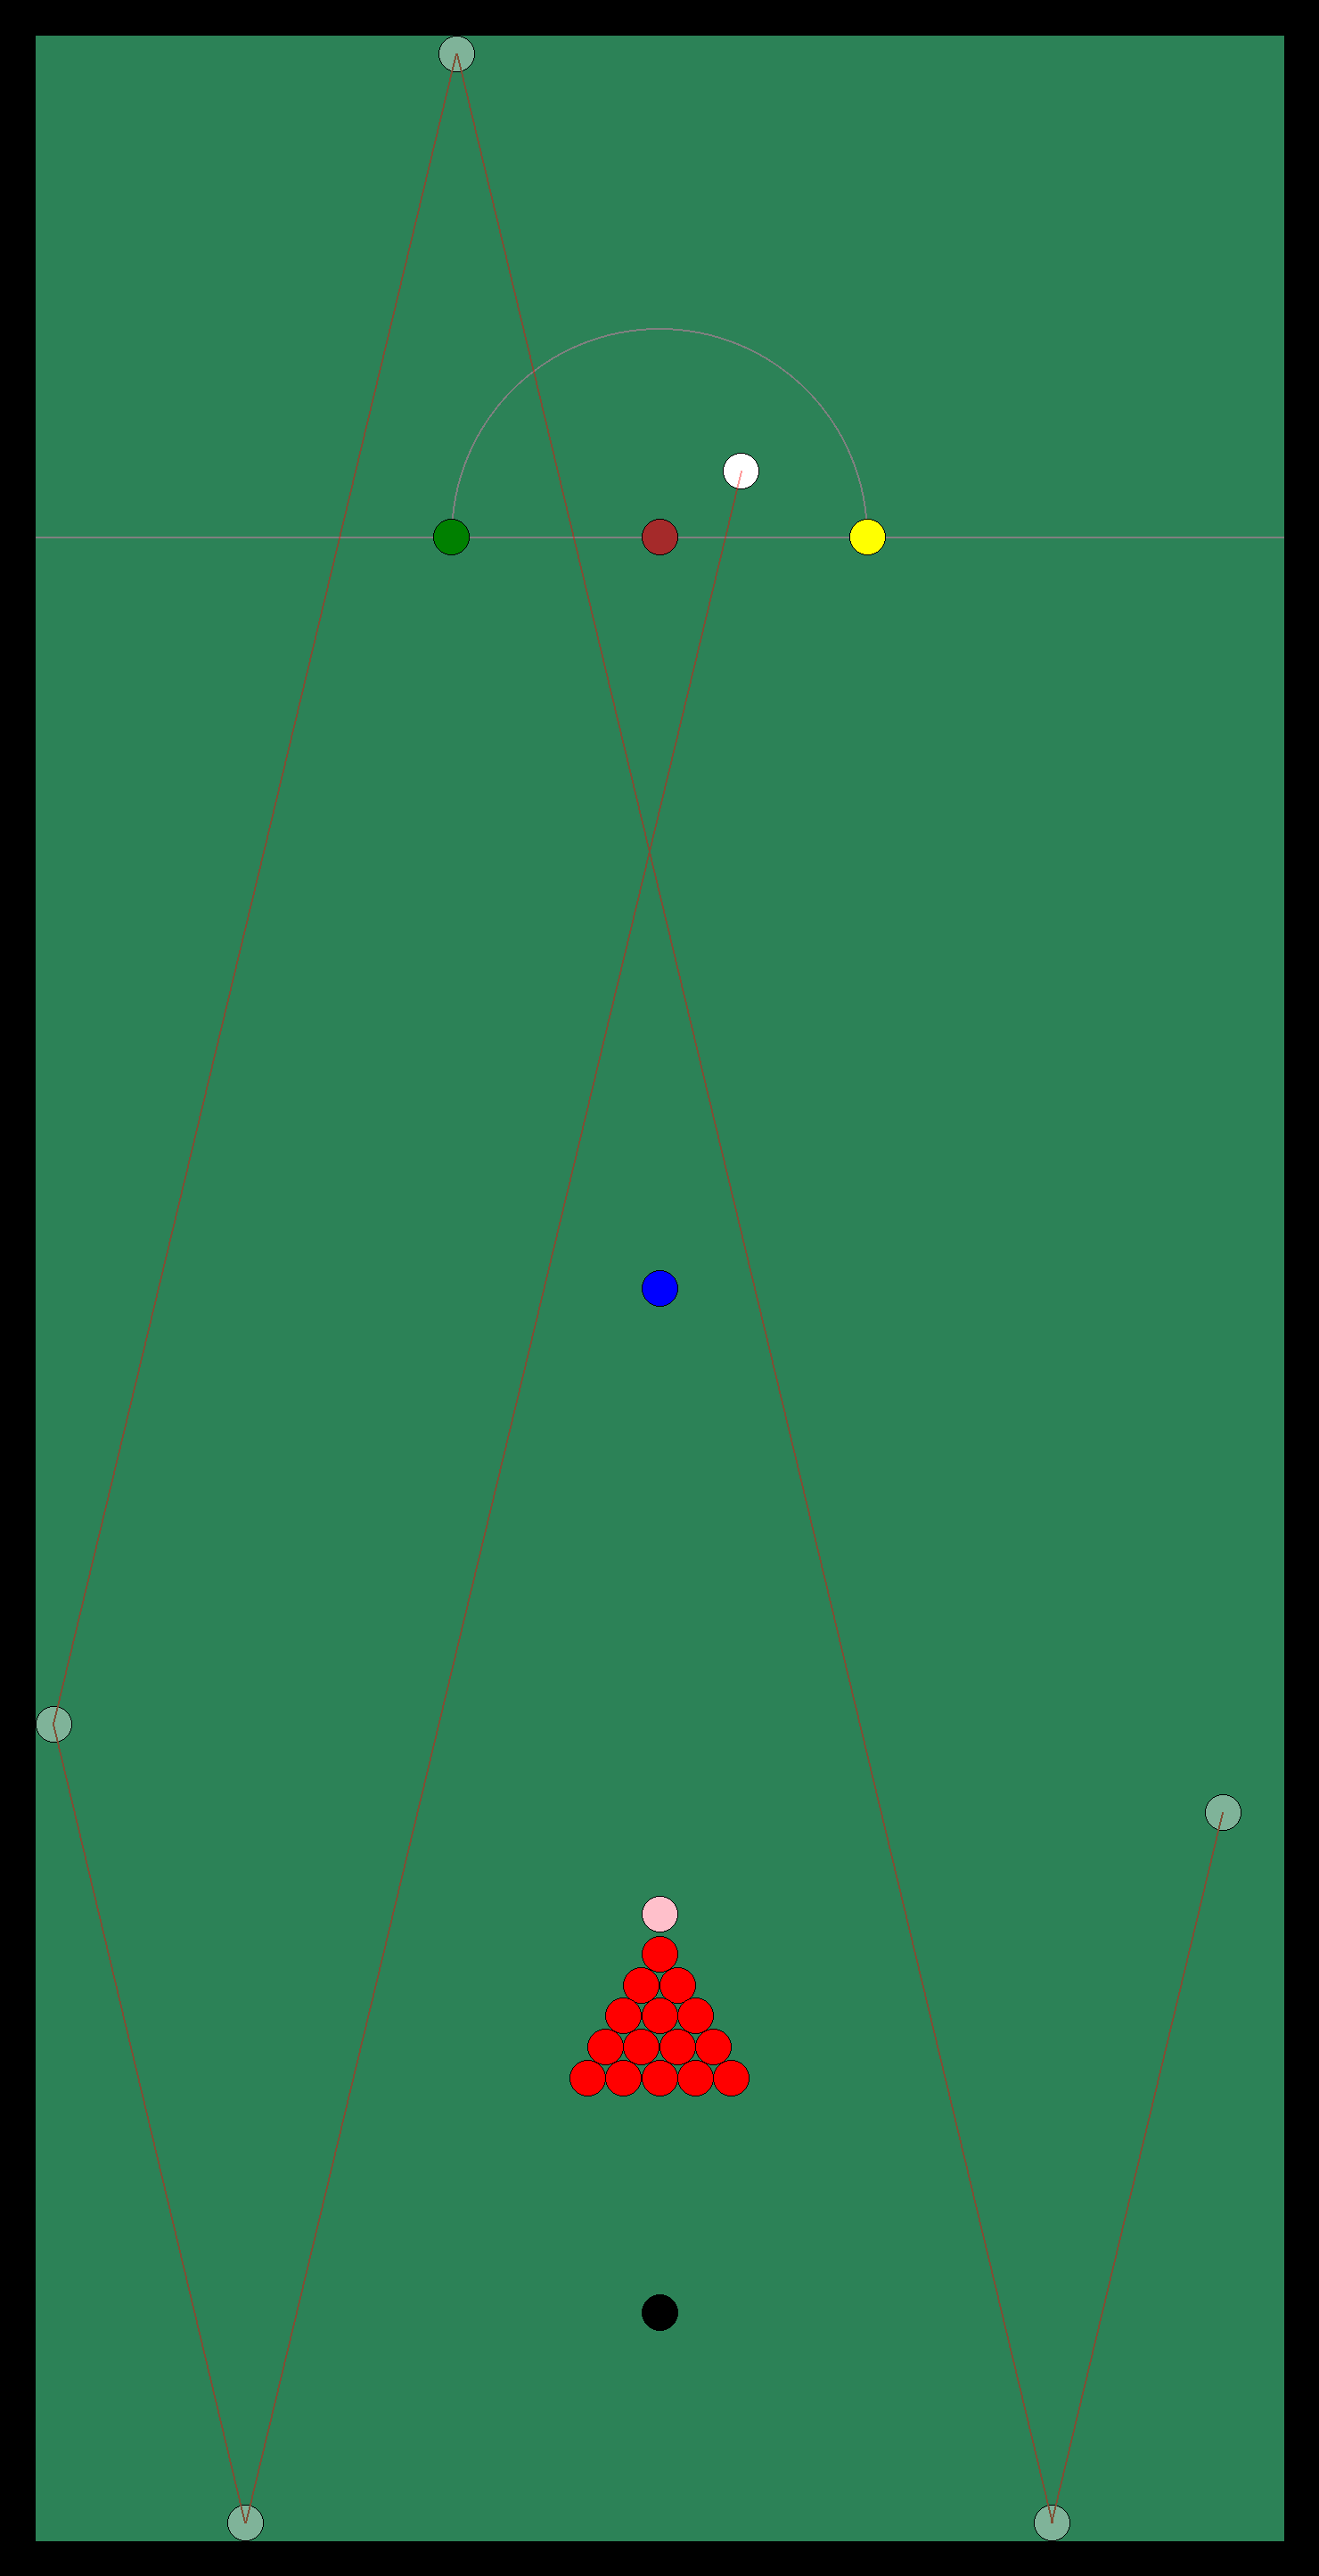
\includegraphics[width=0.7\textwidth]{sample4}
  \caption{Sample 4}
\end{figure}
